\documentclass{bscs}
\usepackage[colorlinks=true, linkcolor=black, urlcolor=blue]{hyperref}
\usepackage{graphicx}

\title{VidSense}
\author{Muhammad Bilal Taha 25132 (Group Lead)\\
         [Muhammad Muaz Arif]\\
         [Muhammad Wasay]\\
         [Syed Bilal Ali]\\
         [Ali Iqbal]}


\begin{document}
\frontmatter
\maketitle

\begin{acknowledgement}
We would like to express our sincere gratitude to our project advisors, Dr Muhammad Saeed and 
Umair Nazir, for their invaluable guidance and support throughout the development of this 
proposal. We also extend our appreciation to our university and department for providing the 
necessary resources and opportunities to pursue this project. 
\end{acknowledgement}

\tableofcontents
\listoftables
\addcontentsline{toc}{chapter}{List of Tables}
\listoffigures
\addcontentsline{toc}{chapter}{List of Figures}
\begin{abbreviations}
    NLP \> Natural Language Processing \\
    AI \> Artificial Intelligence \\
    API \> Application Programming Interface \\
    NLTK \> Natural Language Toolkit \\
\end{abbreviations}
\begin{abstract}
\ VidSense is a video summarization tool designed to improve the accessibility and consumption of lengthy educational and informative videos. The system leverages NLP to provide intelligent video highlights, along with sentiment analysis to offer emotionally enriched summaries. By supporting both Arabic and English, VidSense enhances the user experience with multilingual capabilities. The tool also features a chatbot assisted navigation system, enabling users to interact with and quickly access key moments in the video. VidSense has applications across various fields, including education, research, and content creation, and aims to save users significant time by generating concise video summaries.    
\end{abstract}

\begin{keywords}
Video Summarization, Natural Language Processing, AI-Driven Highlights, Video Content Analysis
\end{keywords}


\mainmatter
\chapter{Introduction}
With the explosion of video content available online, users often struggle to consume lengthy educational or informative videos efficiently. The need to quickly grasp the most relevant parts of educational or informative videos has become paramount, especially for Arabic speaking audiences who face a lack of language support in existing summarization tools.
VidSense aims to address these challenges by providing a robust video summarization tool that offers not only language support for Arabic and English but also integrates a sentiment analysis module. This tool will enable users to view summaries that are emotionally enriched and contextually relevant, allowing for a more engaging and personalized experience.
The app will also include features like chatbot-assisted navigation, multilingual support, and a user-friendly interface, making it a powerful tool for educators, researchers, and general users looking to optimize their video-watching experience.



\section{Objectives}
The primary objectives of this project are:
\begin{itemize}
    \item Generate intelligent video highlights automatically.
    \item Support multilingual capabilities by allowing users to get highlights of the video and chat about the video in Arabic and English languages.
    \item Provide chatbot-assisted navigation across the video for ease of access to required content.
\end{itemize}

\chapter{Literature Review}
The following products exist for video summarization. We discuss why each may leave
some part of our project’s aim unmet.

\begin{table}[h]
    \centering
    \begin{tabular}{|p{3cm}|p{7cm}|p{6cm}|}
        \hline
        \textbf{Application Name} & \textbf{Description} & \textbf{Potential Disadvantages} \\
        \hline
        \href{https://gistly.ly}{Gistly.ly} & The summarizer tool identifies the key points and highlights the most important information, giving you a quick overview of the video’s content. & Does not give option to chat. \\
        \hline
        \href{https://videohighlight.com}{Video Highlight} & Summarizes and takes notes from videos by generating timestamped summaries and transcripts. & Does not give exact moments in the video. Does not generate highlights in the form of video. Timestamps given in response to chat are not clickable. \\
        \hline
        \href{https://notegpt.io}{NoteGPT.io} & Makes notes, summary and highlights of the video, also provides clickable highlights and Arabic support. & Text is summarized but highlights aren’t in the form of video clips. Cannot provide a clip requested. \\
        \hline
    \end{tabular}
    \caption{Comparison of Video Summarization Tools}
\end{table}

\begin{figure}[p]
    \centering
    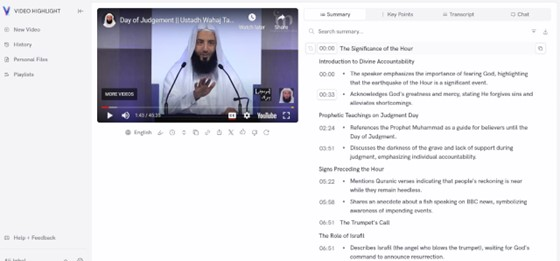
\includegraphics[width=1.1\textwidth]{figure_a.jpg}  
    \caption{Video Highlight fails to give clickable timestamps and doesn’t generate highlights in the form of a video}
    \label{fig:figure1} 
\end{figure}

% Fifth Figure
\begin{figure}[h]
    \centering
    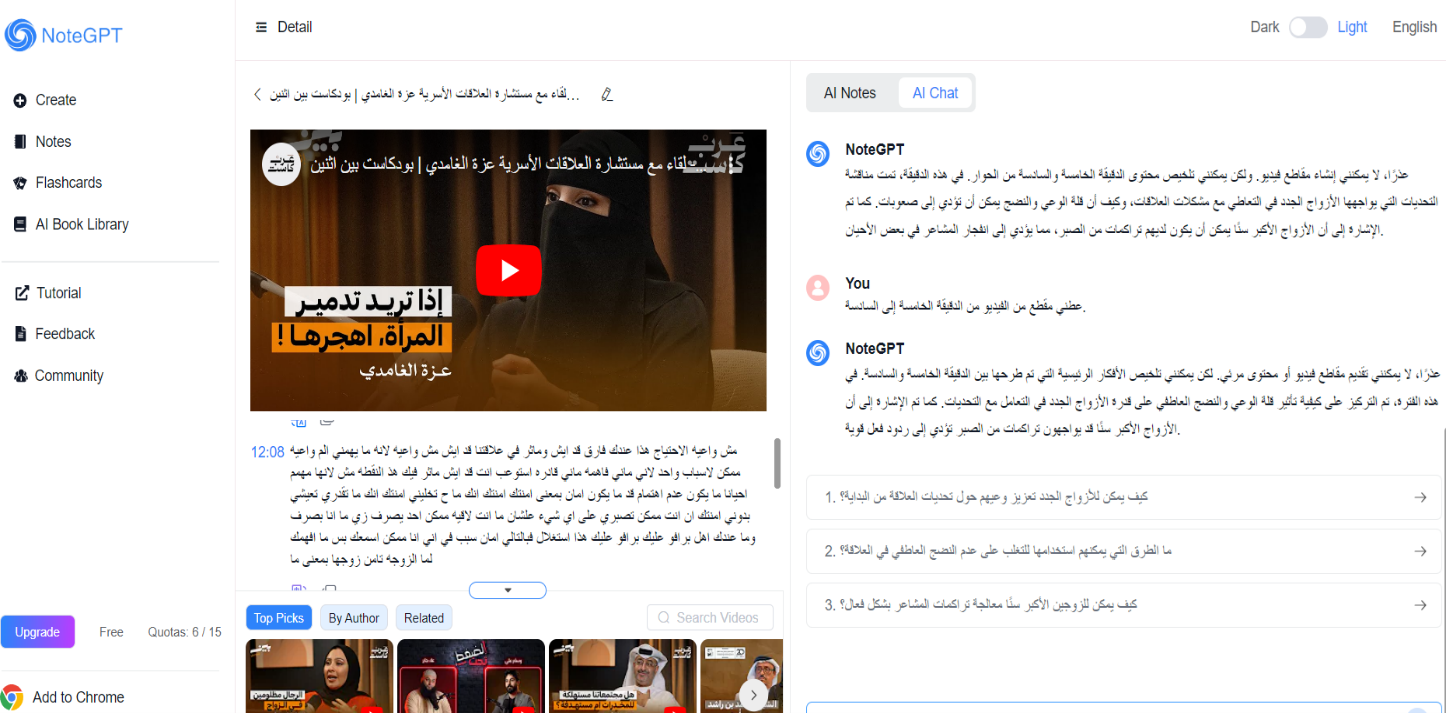
\includegraphics[width=1.1\textwidth]{figure_e.png}  
    \caption{NoteGPT doesn't generate video highlights.}
    \label{fig:figure5}
\end{figure}

% Fourth Figure
\begin{figure}[h]
    \centering
    
\includegraphics[width=1.1\textwidth]{figure_d.png}  
    \caption{Gistly does not have the option to chat with the application}
    \label{fig:figure4}
\end{figure}

\chapter{Proposed System Architecture }

\begin{figure}[h]
    \centering
    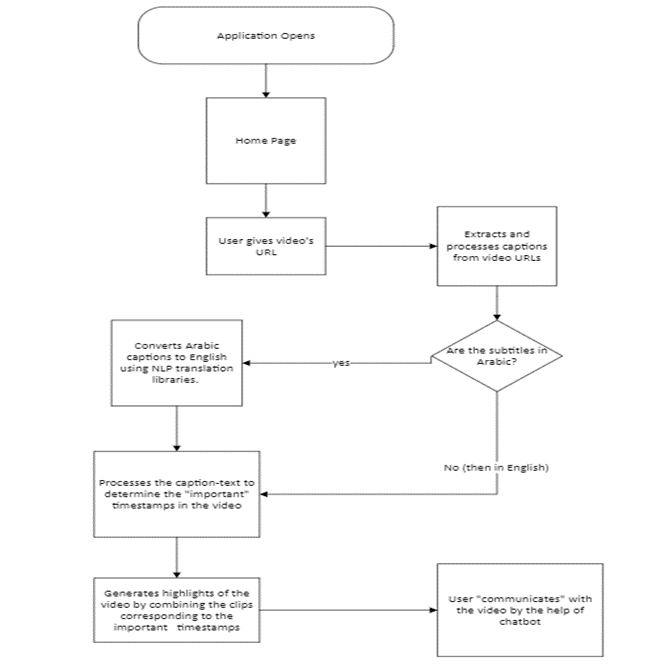
\includegraphics[width=1.0\textwidth]{figure_f.png}  
    \caption{Proposed System Architecture}
    \label{fig:figure4}
\end{figure}

\begin{itemize}
    \item \textbf{Application Opens:} This is the initial step where the user launches the application.
    
    \item \textbf{Home Page:} The user is presented with a homepage where they can interact with the app.
    
    \item \textbf{User Provides Video URL:} The user inputs the URL of the video they want to summarize and analyze.
    
    \item \textbf{Extract and Process Captions from Video URLs:} The system extracts captions from the provided video URL. These captions are the primary text data used for further processing.
    
    \item \textbf{Check if Subtitles are in Arabic:} A decision point checks whether the extracted captions are in Arabic.
    
    \begin{itemize}
        \item If yes, the captions are sent through a translation step.
        \item If no, the captions are directly processed in English.
    \end{itemize}
    
    \item \textbf{Converts Arabic Captions to English Using NLP Translation Libraries:} If the captions are in Arabic, they are translated into English using NLP translation tools.
    
    \item \textbf{Process the Caption-Text to Determine Important Timestamps:} The system analyzes the translated or English captions to identify key timestamps that represent important segments in the video.
    
    \item \textbf{Generate Video Highlights:} Using the identified timestamps, the system generates video highlights by extracting clips corresponding to these important moments.
    
    \item \textbf{User Interaction via Chatbot:} The user can interact with the video summary using a chatbot that helps them navigate the video highlights efficiently.
\end{itemize}

\chapter{Potential Use Cases and Applications}

VidSense has a wide range of applications, including: 
\begin{itemize}
    \item \textbf{Educational Platforms:} Summarizing long lectures and highlighting key emotional moments.
    \item \textbf{Market Analysis:} Analyzing product review videos for sentiment trends. 
    
    \item \textbf{Research and Academia:} Summarizing conference talks and research presentations.

    \item \textbf{Content Creation:} Helping content creators generate quick, sentiment-based video summary.

    
\end{itemize}

\chapter{Impact Assessment}

\begin{itemize}
    \item \textbf{Simplified Access to Key Content:} Users no longer need to watch lengthy videos. They can access key moments and summaries, saving time.
    
    \item \textbf{Language Support:} The app helps Arabic-speaking users by translating subtitles, enhancing accessibility.
    
    \item \textbf{Interactive Chatbot Assistance:} Users can navigate through summaries using a chatbot, improving user experience.
    
    \item \textbf{Time Efficiency:} Saves significant time for users by generating concise summaries.
    
    \item \textbf{Enhanced Learning:} Students and researchers can extract key information quickly, which is ideal for study and research purposes.
    
    \item \textbf{Multi-language Support:} Supports both Arabic and English, catering to a wider audience.
\end{itemize}

\chapter{Future Enhancements}

VidSense can be further enhanced by following features:  
\begin{itemize}
    \item \textbf{Text To Speech:} Reading out the summary of the video content in Arabic and English
language with the tone of speech sensitive to the tone of video i.e. speaker will speak in
excited voice if summarizing the exciting part of the video. (we may use paid tools)
    
    \item \textbf{Notification system:} Notifying the users about the videos according to their interest. 
    
\end{itemize}

\chapter{Technology Stack}

\section{Local Backend}
\textbf{Node.js:} For backend processing and integration.\\
\textbf{React.js or Vue.js:} For frontend UI/UX components.\\
\textbf{Python:} for NLP and AI-related tasks.\\[10pt]

\section{Operating System}
Windows 10/11 or Linux (Ubuntu)\\[10pt]

\section{AI and NLP Technologies}
\textbf{Hugging Face Transformers:} For sentiment analysis and text summarization models.\\
\textbf{spaCy:} For text processing and named entity recognition.\\
\textbf{OpenAI GPT-4 API:} For enhanced text generation and correction of subtitles (optional).\\
\textbf{NLTK:} For text analysis and processing.\\
\textbf{Jais / open-source translation model:} For Arabic to English translation.\\

\chapter{VidSense Ethical and Legal Analysis Report}

VidSense is an innovative video summarization tool aimed at enhancing user experience by
providing quick, relevant, and emotionally enriched video summaries, specifically tailored for
Arabic and English-speaking audiences. This report evaluates VidSense from ethical and legal
perspectives, highlighting potential risks and societal implications. 

\section{I-2: Casuistry}

\subsection{Comparison of Similar Tools}

VidSense distinguishes itself from existing video summarization tools, such as NoteGPT.io,
Gist.ly, and Video Highlight, by integrating sentiment analysis, Arabic support, and a chatbot
interface. Below is a comparative overview: 

\begin{itemize}
    \item \textbf{NoteGPT.io:} Offers clickable timestamps for key highlights and limited Arabic support but lacks the ability to generate video clips. 
    
    \item \textbf{Gist.ly:} Provides text-based summaries but does not feature chat capabilities or
multilingual support, limiting its accessibility.

    \item \textbf{Video Highlight:} Generates timestamped summaries but fails to create video clips and lacks interactive chatbot features.
\end{itemize}

\subsection{Ethical Considerations}

\begin{itemize}
    \item \textbf{Data Privacy:} VidSense extracts captions from user-uploaded video URLs, raising
concerns about handling personal or sensitive information. To mitigate risks, it must
ensure strong data anonymization and security protocols, taking lessons from Gist.ly’s
shortcomings in data security.  
    
    \item \textbf{Bias in Sentiment Analysis:} The sentiment analysis feature, while beneficial, may
introduce biases in content interpretation, especially given cultural differences between Arabic and English speakers. Continuous refinement of machine learning models is
necessary to address these biases. 

    \item \textbf{Inclusivity:} While VidSense’s support for Arabic reflects a commitment to inclusivity, itmust ensure effective functionality across various Arabic dialects. Engaging with diverse Arabic-speaking communities for feedback will be crucial.

\end{itemize}
    
\subsection{Lessons for VidSense}

\begin{itemize}
    \item \textbf{User Privacy:} Implement robust encryption measures and comply with global data
protection regulations like GDPR to protect user data. 
    
    \item \textbf{Cultural Sensitivity in Sentiment Analysis:}  Develop sentiment analysis models that accurately reflect cultural expressions and emotions to avoid misinterpretations.  

    \item \textbf{Inclusivity in Language Support:} Collect user feedback from a wide range of Arabic
speakers to improve translation accuracy and sentiment recognition.

\end{itemize}

\section{I-3: Similar Projects & Legal, Societal Considerations}

\subsection{Similar Projects}

VidSense can learn from similar tools regarding societal and legal challenges:

\begin{itemize}
    \item \textbf{NoteGPT.io:} Strengths in providing text summaries but lacks interactive elements. 
    
    \item \textbf{Gist.ly:} Quick summaries but limited by lack of user interaction and multilingual
capabilities.  

    \item \textbf{Video Highlight:} Good at timestamping but misses out on generating video clips.

\end{itemize}

\subsection{Legal Considerations}

\begin{itemize}
    \item \textbf{Copyright and Fair Use:} VidSense must navigate copyright laws to avoid infringement when summarizing content. Implementing a licensing framework and prioritizing public
domain or Creative Commons content will be essential. 
    
    \item \textbf{Data Protection:} Compliance with data protection laws like GDPR is crucial. VidSense should ensure that user data is encrypted and anonymized and obtain explicit user consent for data processing.  

\end{itemize}

\subsection{Societal Considerations}

\begin{itemize}
    \item \textbf{Educational Impact:} VidSense can enhance educational engagement but risks losing
critical context in summaries. Users should have access to full videos alongside
summaries. 
    
    \item \textbf{Risk of Misinformation:} Sentiment analysis can inadvertently distort the original
content, potentially leading to misinformation. Safeguards, such as fact-checking tools,
are necessary to maintain content integrity.
\end{itemize}

\section{S-2: Expanding the Circle of Stakeholders and Identifying Dual-Use Cases}

\subsection{Expanding the Circle of Stakeholders}

Beyond casual viewers, VidSense should consider the following stakeholders:

\begin{itemize}
    \item \textbf{Content Creators:} Utilize VidSense to generate summaries that improve content
accessibility. 
    
    \item \textbf{Educators and Researchers:} Summarize educational content for quicker review. 

    \item \textbf{Business and Marketing Professionals:} Analyze customer sentiment through video
content. 

    \item \textbf{Public Policy and Social Organizations:} Summarize key information from public
speeches and documentaries.  

\end{itemize}

\subsection{Dual-Use Cases}

VidSense features may be applied in potentially harmful ways: 

\begin{itemize}
    \item \textbf{Misinformation and Propaganda:} Misuse in distorting original video messages through biased summarization. 
    
    \item \textbf{Surveillance:} Potential misuse for analyzing sensitive videos, leading to privacy violations.  

    \item \textbf{Content Moderation:}  Risk of unfair censorship in moderation systems.

    \item \textbf{Corporate Monitoring:} Potential privacy concerns if used to monitor employee
behavior.
    
\end{itemize}

\section{S-3: Legal, Environmental, Public Health, and Cultural Considerations}

\subsection{Legal Considerations}

\begin{itemize}
    \item \textbf{Copyright and Intellectual Property:} Ensure compliance with copyright laws by
processing only appropriately licensed content. 
    
    \item \textbf{Data Privacy:}  Implement strong data protection measures to comply with laws like GDPR.   

\end{itemize}

\subsection{Environmental Considerations}

\begin{itemize}
    \item \textbf{Energy Consumption:} Address the environmental impact of processing large video files by using energy-efficient servers and considering carbon offset programs.  
    
    \item \textbf{Server Infrastructure:} Optimize for lower energy consumption and consider sustainable hosting options.

\end{itemize}

\subsection{Public Health Considerations}

\begin{itemize}
    \item \textbf{Mental Health:} Summarize content from mental health resources, ensuring sentiment analysis does not misinterpret sensitive emotional content. 
    
    \item \textbf{Health Misinformation:}  Implement validation mechanisms to prevent the spread of
inaccurate health information.

\end{itemize}

\chapter{References}

Apostolidis, Evlampios, Eleni Adamantidou, Alexandros I. Metsai, Vasileios Mezaris, and
Ioannis Patras. 2021. “Video Summarization Using Deep Neural Networks: A Survey.
Proceedings of the IEEE International Conference on Image Processing”\\
\url{https://doi.org/10.48550/arXiv.2101.06072}\\

Meena, Preeti, Himanshu Kumar, and Sandeep Kumar Yadav. 2021. “A Review on Video
Summarization Techniques.”. Department of Electrical Engineering, Indian Institute of
Technology.\\
\url{https://doi.org/10.1016/j.engappai.2022.105667}\\

Saini, P., Kumar, K., Kashid, S., et al. 2023. "Video Summarization Using Deep Learning
Techniques: A Detailed Analysis and Investigation." \\
\url{https://link.springer.com/article/10.1007/s10462-023-10444-0}\\

Ul Haq, Hafiz Burhan, Muhammad Asif, Maaz Bin Ahmad, Rehan Ashraf, and Toqeer
Mahmood. Year. “An Effective Video Summarization Framework Based on the Object of
Interest Using Deep Learning.” \\
\url{https://doi.org/10.1155/2022/7453744}

\end{document}
